\documentclass{article}
\usepackage[utf8]{inputenc}
\usepackage[a4paper, total={6.5in, 9.5in}]{geometry}
\usepackage{graphicx} % Required for inserting images
\usepackage{enumitem}
\usepackage{booktabs,adjustbox}
\usepackage{multirow,multicol}
\usepackage{xcolor}
\usepackage{array,caption}
\usepackage{amssymb,amsmath}
\usepackage{ragged2e}
\usepackage{tikz,circuitikz}
\usepackage{titling}
\usepackage{hyperref}
\usepackage{tkz-euclide,subfigure}
\usepackage{subcaption}
\usepackage{nameref}
\captionsetup{font=Large}
\usepackage{algorithm}
\usepackage{algorithmic}
\usetikzlibrary{shapes.geometric}
\usetikzlibrary{shapes,arrows,positioning,patterns,matrix,circuits.logic.IEC, calc}
\usepackage{pgfplots}
\pgfplotsset{compat=newest}
\usepgfplotslibrary{fillbetween,statistics}

\graphicspath{ {./Img/} }

\definecolor{blizzardblue}{rgb}{0.67, 0.9, 0.93}
\definecolor{bittersweet}{rgb}{1.0, 0.44, 0.37}
\definecolor{caribbeangreen}{rgb}{0.0, 0.8, 0.6}
\definecolor{carnationpink}{rgb}{1.0, 0.65, 0.79}
\definecolor{capri}{rgb}{0.0, 0.75, 1.0}
\definecolor{green(pigment)}{rgb}{0.0, 0.65, 0.31}
\definecolor{grannysmithapple}{rgb}{0.66, 0.89, 0.63}

% set spacing in tables
\setlength{\tabcolsep}{12pt}
\renewcommand{\arraystretch}{1.5}

\pretitle{\linespread{1.5}\Large}
\posttitle{\vspace{10mm}}

\title{
\begin{center}
\begin{figure}[!h]
    \centering
    
\includegraphics[scale = 0.75]{Img/buetlogo.png}
\end{figure}
CSE 300\\
Technical Writing and Presentation Sessional\\
Report: Maximum Bipartite Matching\\
Lab Section - A1\\
Group - 09\\
9th March, 2024
\end{center}
}
\author{}
\date{}

\begin{document}

\maketitle

\raggedright
\Large{Members of the Group:\par}
\Large{
\begin{enumerate}[label = \roman*.]
    \item 2005012 - Abrar Jahin Sarker
    \item 2005017 - Abdullah  Muhammed  Amimul Ehsan
    \item 2005020 - Mostafa Rifat Tazwar
\end{enumerate}
}
\newpage
\tableofcontents
\newpage
\section{Introduction}
\Large
The concept of maximum bipartite matching, a fundamental problem in graph theory, holds significant relevance across diverse fields due to its ability to model various real-world scenarios. Bipartite graphs serve as the foundational structure for this problem. In essence, a maximum bipartite matching seeks to pair elements from one subset with elements from the other subset in such a way that maximizes the number of paired elements. From applications in network flow optimization, job scheduling, and medical residency programs to its role in solving matching problems in societal contexts like marriage and kidney exchange programs, the utility of maximum bipartite matching extends across numerous domains, making it a subject of continued research and innovation.  
\subsection{Definitions}
\subsubsection{\large Bipartite Graph}
\Large
A bipartite graph is one whose vertices can be split into two independent groups U,V such that \textbf{every edge connects vertices of different groups.} \\
\vspace{10mm}
\begin{figure}[H]
    \centering
    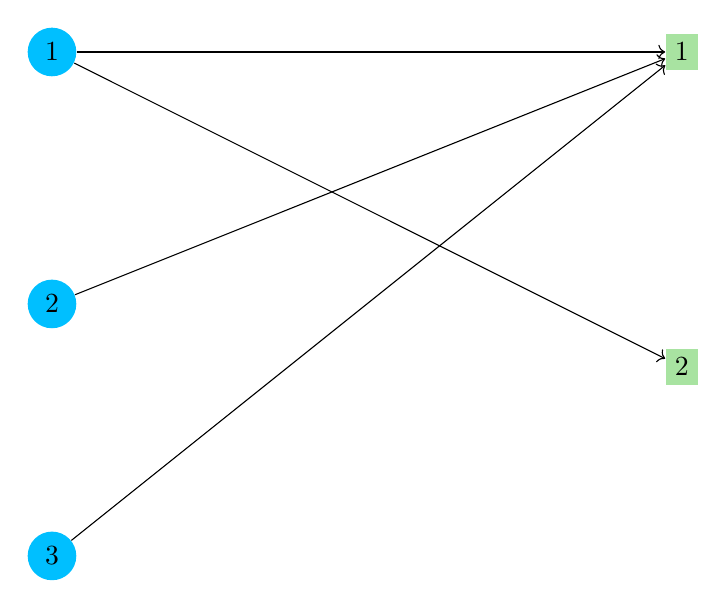
\begin{tikzpicture}[scale=4] 
        % 
        \node[fill=capri, circle] (b1) at (0,0) {1};
        \node[fill=capri, circle] (b2) at (0,-0.8) {2};
        \node[fill=capri, circle] (b3) at (0,-1.6) {3};
        
        % Girl
        \node[fill=grannysmithapple, rectangle] (g1) at (2,0) {1};
        \node[fill=grannysmithapple, rectangle] (g2) at (2,-1) {2};
        
        % Potential Pairs
        \draw[->] (b1) -- (g1);
        \draw[->] (b1) -- (g2);
        \draw[->] (b2) -- (g1);
        \draw[->] (b3) -- (g1);
        

    \end{tikzpicture}
    \caption{Visualization of bipartite graph}
\end{figure}
\newpage
\large \textbf{Properties of a Bipartite graph}\\
\Large
\begin{itemize}
    \item[-] There can \underline{not} be any edge between any two vertices of U or any two vertices of V .\\
    \item[-] The graph is \textcolor{blue}{two colourable} and doesn't have \textcolor{red}{cycles of odd length}.
\end{itemize}


\begin{figure}[H]
    \centering
    \begin{tabular}{c c}
        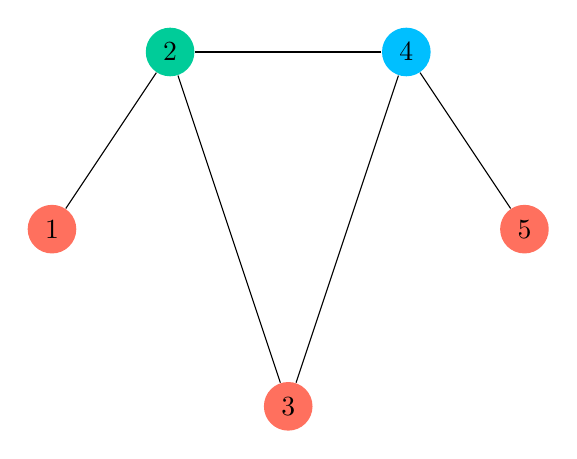
\begin{tikzpicture}[scale=1.5]
        
        
            \node[fill=bittersweet, circle] (r1) at (-0.75,0) {1} ;
            \node[fill=bittersweet, circle] (r3) at (1.25,-1.5) {3} ;
            \node[fill=bittersweet, circle] (r5) at (3.25,0) {5} ;
            \node[fill=caribbeangreen, circle] (g2) at (0.25,1.5) {2} ;
            \node[fill=capri, circle] (g4) at (2.25,1.5) {4} ;    
            
            \draw[-] (r1) -- (g2) ;
            \draw[-] (g2) -- (r3);
            \draw[-] (r3) -- (g4);
            \draw[-] (g4) -- (g2);
            \draw[-] (g4) -- (r5);
        
        
        
        \end{tikzpicture} & 
    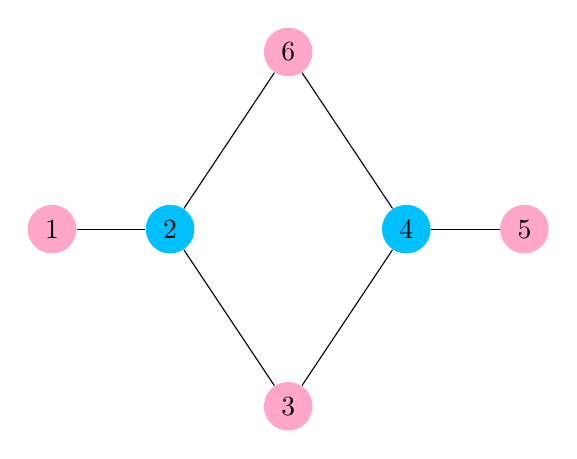
\begin{tikzpicture}[scale = 1.5]
        \node[fill=carnationpink, circle] (p1) at (-0.75,0) {1} ;
        \node[fill=carnationpink, circle] (p3) at (1.25,-1.5) {3} ;
        \node[fill=carnationpink, circle] (p6) at (1.25,1.5) {6} ;
        \node[fill=carnationpink, circle] (p5) at (3.25,0) {5} ;
        \node[fill=capri, circle] (b2) at (0.25,0) {2} ;
        \node[fill=capri, circle] (b4) at (2.25,0) {4} ;    
        
        \draw[-] (p1) -- (b2) ;
        \draw[-] (b2) -- (p3);
        \draw[-] (b2) -- (p6);
        \draw[-] (b4) -- (p3);
        \draw[-] (b4) -- (p6);
        \draw[-] (b4) -- (p5);
    \end{tikzpicture} \\
    Odd length cycle & Even length cycle \\
    Not 2 colorable & 2 colorable \\ 
    \textcolor{red}{Not a bipartite graph} &  \textcolor{caribbeangreen}{Bipartite graph}
    \end{tabular}
    \caption{Comparison between Bipartite and Non-bipartite graph}
\end{figure}

\subsubsection{\large Maximum Matching}
Given a bipartite graph, a matching is a subset of the edges for which \textbf{every vertex belongs to exactly one of the edges}. \par

And, a maximum matching is a matching of \textbf{maximum number of edges}. In a maximum matching, if any edge is added to it, it is no longer a matching.

\section{The Problem}
\textit{
Given a bipartite graph $G = (A \cup B, E)$, find an \{ $S \subseteq A \times B$ : $S$ is a matching and is as large as possible.} \} \cite{kleinberg2006algorithm}

\newpage

\section{Scenario}
In a picnic,there are 5 people and 5 food items.Some people express interest in some of the items.How can we satisfy \textbf{maximum number of people} while wasting \textbf{minimum number of items}?

\section{Greedy Approach}
Greedy approach seeks to find the \textbf{first available item} among the items in which the person is interested in and assigns that item to the person. Here's a simulation for the above scenario :- 

\begin{table}[!h]
    \centering
    \begin{tabular}{ccc}
      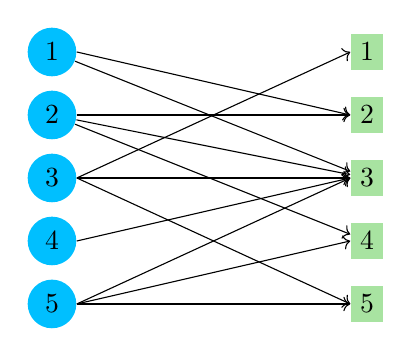
\begin{tikzpicture} 
            % 
            \node[fill=capri, circle] (p1) at (0,0) {1};
            \node[fill=capri, circle] (p2) at (0,-0.8) {2};
            \node[fill=capri, circle] (p3) at (0,-1.6) {3};
             \node[fill=capri, circle] (p4) at (0,-2.4) {4};
            \node[fill=capri, circle] (p5) at (0,-3.2) {5};
             
            
            
            % 
            \node[fill=grannysmithapple, rectangle] (f1) at (4,0) {1};
            \node[fill=grannysmithapple, rectangle] (f2) at (4,-0.8) {2};
            \node[fill=grannysmithapple, rectangle] (f3) at (4,-1.6) {3};
            \node[fill=grannysmithapple, rectangle] (f4) at (4,-2.4) {4};
            \node[fill=grannysmithapple, rectangle] (f5) at (4,-3.2) {5};
            
            % Potential Pairs
            \draw[->] (p1.east) -- (f2.west);
            \draw[->] (p1) -- (f3);
            \draw[->] (p2) -- (f2);
            \draw[->] (p2) -- (f3);
            \draw[->] (p2) -- (f4);
             \draw[->] (p3.east) -- (f1.west);
              \draw[->] (p3.east) -- (f3.west);
               \draw[->] (p3.east) -- (f5.west);
                \draw[->] (p4.east) -- (f3.west);
                  \draw[->] (p5.east) -- (f3.west);
               \draw[->] (p5.east) -- (f5.west);
                \draw[->] (p5.east) -- (f4.west);
            
            
            

        \end{tikzpicture} & 
        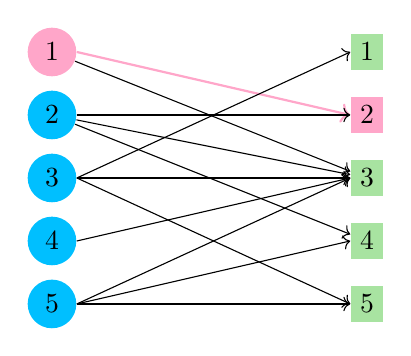
\begin{tikzpicture} 
            % 
            \node[fill=carnationpink, circle] (p1) at (0,0) {1};
            \node[fill=capri, circle] (p2) at (0,-0.8) {2};
            \node[fill=capri, circle] (p3) at (0,-1.6) {3};
             \node[fill=capri, circle] (p4) at (0,-2.4) {4};
            \node[fill=capri, circle] (p5) at (0,-3.2) {5}; 
            
            
            % 
            \node[fill=grannysmithapple, rectangle] (f1) at (4,0) {1};
            \node[fill=carnationpink, rectangle] (f2) at (4,-0.8) {2};
            \node[fill=grannysmithapple, rectangle] (f3) at (4,-1.6) {3};
            \node[fill=grannysmithapple, rectangle] (f4) at (4,-2.4) {4};
            \node[fill=grannysmithapple, rectangle] (f5) at (4,-3.2) {5};
        
            
            % Potential Pairs
           \draw[carnationpink,thick,->] (p1.east) --  (f2.west);
            \draw[->] (p1) -- (f3);
            \draw[->] (p2) -- (f2);
            \draw[->] (p2) -- (f3);
            \draw[->] (p2) -- (f4);
             \draw[->] (p3.east) -- (f1.west);
              \draw[->] (p3.east) -- (f3.west);
               \draw[->] (p3.east) -- (f5.west);
                \draw[->] (p4.east) -- (f3.west);
                  \draw[->] (p5.east) -- (f3.west);
               \draw[->] (p5.east) -- (f5.west);
                \draw[->] (p5.east) -- (f4.west);
            
            
            

        \end{tikzpicture} & 
        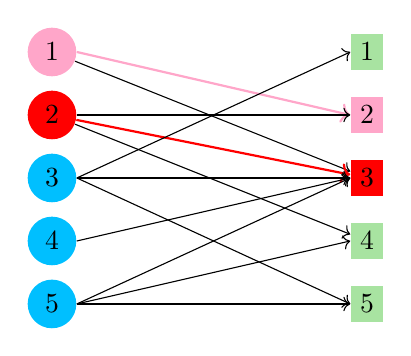
\begin{tikzpicture} 
            % 
            \node[fill=carnationpink, circle] (p1) at (0,0) {1};
            \node[fill=red, circle] (p2) at (0,-0.8) {2};
            \node[fill=capri, circle] (p3) at (0,-1.6) {3};
             \node[fill=capri, circle] (p4) at (0,-2.4) {4};
            \node[fill=capri, circle] (p5) at (0,-3.2) {5};
             
            
            
            % 
            \node[fill=grannysmithapple, rectangle] (f1) at (4,0) {1};
            \node[fill=carnationpink, rectangle] (f2) at (4,-0.8) {2};
            \node[fill=red, rectangle] (f3) at (4,-1.6) {3};
            \node[fill=grannysmithapple, rectangle] (f4) at (4,-2.4) {4};
            \node[fill=grannysmithapple, rectangle] (f5) at (4,-3.2) {5};
            
            % Potential Pairs
           \draw[carnationpink,thick,->] (p1.east) --  (f2.west);
            \draw[->] (p1) -- (f3);
            \draw[->] (p2) -- (f2);
            \draw[red,thick,->] (p2) -- (f3);
            \draw[->] (p2) -- (f4);
             \draw[->] (p3.east) -- (f1.west);
              \draw[->] (p3.east) -- (f3.west);
               \draw[->] (p3.east) -- (f5.west);
                \draw[->] (p4.east) -- (f3.west);
                  \draw[->] (p5.east) -- (f3.west);
               \draw[->] (p5.east) -- (f5.west);
                \draw[->] (p5.east) -- (f4.west);
            
            
            

        \end{tikzpicture} \\
        (a) & (b) & (c) \\ \hline
        & & \\
        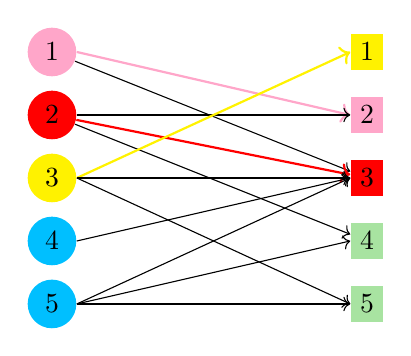
\begin{tikzpicture} 
            % 
            \node[fill=carnationpink, circle] (p1) at (0,0) {1};
            \node[fill=red, circle] (p2) at (0,-0.8) {2};
            \node[fill=yellow, circle] (p3) at (0,-1.6) {3};
             \node[fill=capri, circle] (p4) at (0,-2.4) {4};
            \node[fill=capri, circle] (p5) at (0,-3.2) {5};
             
            
            
            % 
            \node[fill=yellow, rectangle] (f1) at (4,0) {1};
            \node[fill=carnationpink, rectangle] (f2) at (4,-0.8) {2};
            \node[fill=red, rectangle] (f3) at (4,-1.6) {3};
            \node[fill=grannysmithapple, rectangle] (f4) at (4,-2.4) {4};
            \node[fill=grannysmithapple, rectangle] (f5) at (4,-3.2) {5};
            
            % Potential Pairs
           \draw[carnationpink,thick,->] (p1.east) --  (f2.west);
            \draw[->] (p1) -- (f3);
            \draw[->] (p2) -- (f2);
            \draw[red,thick,->] (p2) -- (f3);
            \draw[->] (p2) -- (f4);
             \draw[yellow,thick,->] (p3.east) -- (f1.west);
              \draw[->] (p3.east) -- (f3.west);
               \draw[->] (p3.east) -- (f5.west);
                \draw[->] (p4.east) -- (f3.west);
                  \draw[->] (p5.east) -- (f3.west);
               \draw[->] (p5.east) -- (f5.west);
                \draw[->] (p5.east) -- (f4.west);
            
            
            

        \end{tikzpicture} &
        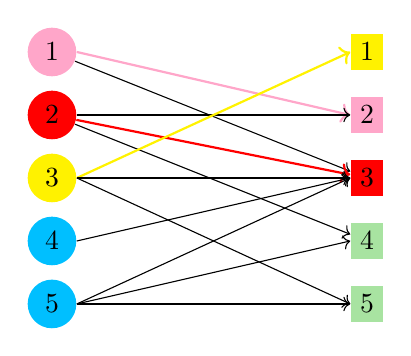
\begin{tikzpicture} 
            % 
            \node[fill=carnationpink, circle] (p1) at (0,0) {1};
            \node[fill=red, circle] (p2) at (0,-0.8) {2};
            \node[fill=yellow, circle] (p3) at (0,-1.6) {3};
             \node[fill=capri, circle] (p4) at (0,-2.4) {4};
            \node[fill=capri, circle] (p5) at (0,-3.2) {5};
             
            
            
            % 
            \node[fill=yellow, rectangle] (f1) at (4,0) {1};
            \node[fill=carnationpink, rectangle] (f2) at (4,-0.8) {2};
            \node[fill=red, rectangle] (f3) at (4,-1.6) {3};
            \node[fill=grannysmithapple, rectangle] (f4) at (4,-2.4) {4};
            \node[fill=grannysmithapple, rectangle] (f5) at (4,-3.2) {5};
            
            % Potential Pairs
           \draw[carnationpink,thick,->] (p1.east) --  (f2.west);
            \draw[->] (p1) -- (f3);
            \draw[->] (p2) -- (f2);
            \draw[red,thick,->] (p2) -- (f3);
            \draw[->] (p2) -- (f4);
             \draw[yellow,thick,->] (p3.east) -- (f1.west);
              \draw[->] (p3.east) -- (f3.west);
               \draw[->] (p3.east) -- (f5.west);
                \draw[->] (p4.east) -- (f3.west);
                  \draw[->] (p5.east) -- (f3.west);
               \draw[->] (p5.east) -- (f5.west);
                \draw[->] (p5.east) -- (f4.west);
            
            
            

        \end{tikzpicture} &
        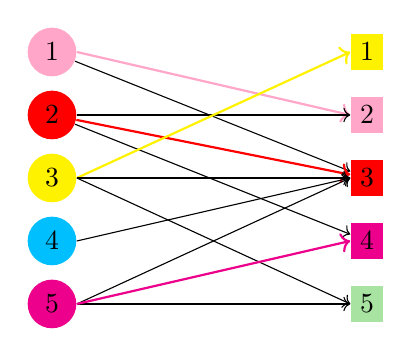
\begin{tikzpicture} 
            % 
            \node[fill=carnationpink, circle] (p1) at (0,0) {1};
            \node[fill=red, circle] (p2) at (0,-0.8) {2};
            \node[fill=yellow, circle] (p3) at (0,-1.6) {3};
             \node[fill=capri, circle] (p4) at (0,-2.4) {4};
            \node[fill=magenta, circle] (p5) at (0,-3.2) {5};
             
            
            
            % 
            \node[fill=yellow, rectangle] (f1) at (4,0) {1};
            \node[fill=carnationpink, rectangle] (f2) at (4,-0.8) {2};
            \node[fill=red, rectangle] (f3) at (4,-1.6) {3};
            \node[fill=magenta, rectangle] (f4) at (4,-2.4) {4};
            \node[fill=grannysmithapple, rectangle] (f5) at (4,-3.2) {5};
            
            % Potential Pairs
           \draw[carnationpink,thick,->] (p1.east) --  (f2.west);
            \draw[->] (p1) -- (f3);
            \draw[->] (p2) -- (f2);
            \draw[red,thick,->] (p2) -- (f3);
            \draw[->] (p2) -- (f4);
             \draw[yellow,thick,->] (p3.east) -- (f1.west);
              \draw[->] (p3.east) -- (f3.west);
               \draw[->] (p3.east) -- (f5.west);
                \draw[->] (p4.east) -- (f3.west);
                  \draw[->] (p5.east) -- (f3.west);
               \draw[->] (p5.east) -- (f5.west);
                \draw[magenta,thick,->] (p5.east) -- (f4.west);
            
            
            

        \end{tikzpicture} 
        \\
        (d) & (e) & (f) \\ \hline
    \end{tabular}
    \caption*{
    a) We define the problem using a graph, where any \textcolor{blue}{blue} vertex represents a person to whom no item has been assigned and any \textcolor{caribbeangreen}{green} vertex represents an available item. Edges from a person to an item depicts their interest in that item.
    \\ b) Person 1 initiates the process by selecting the first available item (item 2).
	\\ c) Person 2's only viable option is item 3, as item 2 has already been chosen.
	\\ d) Person 3 selects item 1.
	\\ e) Person 4 cannot be assigned an item, as all options previously chosen by them have been allocated.
	\\ f) Person 5 discovers that item 4 is available for selection.
	}
    \label{tab:greedy_approch}
\end{table}
\textit{Bipartite matching : }  \{(1, 2), (2, 3), (3, 1), (5, 4)\}\\

Although greedy provides us with a valid matching , it is not maximal.












\section{Reduction to a Known Problem}


            % Text column
            \begin{itemize}
                \item Given an instance of bipartite matching
                
                \item Reduce it to Max Flow Problem.
            
                \item 
Where the solution to the
network 
flow problem can
easily be used to find the
solution to the bipartite
matching.
            \end{itemize}
    
        
 
            % Flowchart column
            \begin{figure}[H]
                \centering
		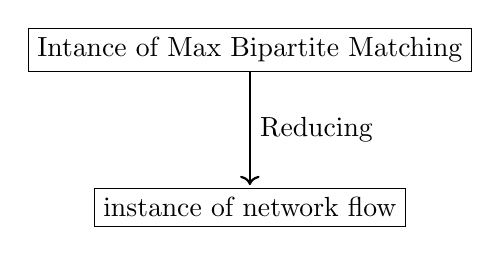
\begin{tikzpicture} [shorten >=1pt,node distance=2cm,auto]
                    % Nodes
                    \node[draw,rectangle] (A1) {Intance of Max Bipartite Matching};
                    \node[draw,rectangle] (B5) [below of=A1] {instance of network flow};
                
                    % Arrow
                    \draw[black,thick,->] (A1.south) -- node[midway, right] {Reducing} (B5.north);
                \end{tikzpicture}
                \caption{Approach to solve}
            \end{figure}



\section{Steps of Reduction}

\subsection{ Make all the edges directed}

Make all the edges directed if not and add 0 flow and 1 capacity for all edges, expressed as 0/1 in Flow/Capacity format.

\begin{figure}[H]
\begin{center}
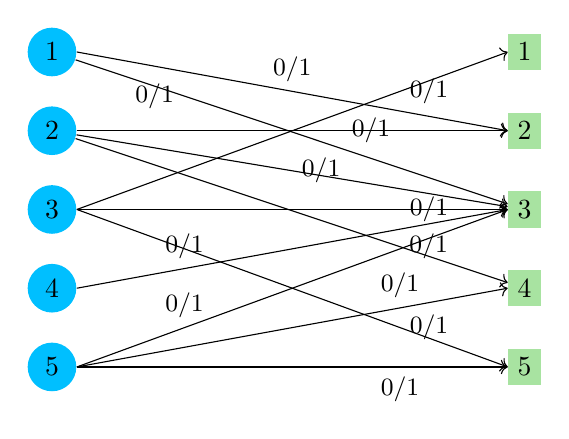
\begin{tikzpicture}
    \node[fill=capri, circle] (p1) at (0,0) {1};
    \node[fill=capri, circle] (p2) at (0,-1) {2};
    \node[fill=capri, circle] (p3) at (0,-2) {3};
    \node[fill=capri, circle] (p4) at (0,-3) {4};
    \node[fill=capri, circle] (p5) at (0,-4) {5};
     
    \node[fill=grannysmithapple, rectangle] (f1) at (6,0) {1};
    \node[fill=grannysmithapple, rectangle] (f2) at (6,-1) {2};
    \node[fill=grannysmithapple, rectangle] (f3) at (6,-2) {3};
    \node[fill=grannysmithapple, rectangle] (f4) at (6,-3) {4};
    \node[fill=grannysmithapple, rectangle] (f5) at (6,-4) {5};
    
    % Potential Pairs
    \draw[->] (p1.east)--node[midway,above,font=\small]{0/1}  (f2.west);
    \draw[->] (p1) -- node[near start,left,font=\small]{0/1}  (f3);
    \draw[->] (p2) -- node[near end,left,font=\small]{0/1}  (f2);
    \draw[->] (p2) -- node[midway,right,font=\small]{0/1}  (f3);
    \draw[->] (p2) -- node[near end,right,font=\small]{0/1} (f4);
    \draw[->] (p3.east) -- node[near end,right,font=\small]{0/1}  (f1.west);
    \draw[->] (p3.east) -- node[near end,right,font=\small]{0/1}  (f3.west);
    \draw[->] (p3.east) -- node[near end,right,font=\small]{0/1}  (f5.west);
    \draw[->] (p4.east) -- node[near start,above,font=\small]{0/1}  (f3.west);
    \draw[->] (p5.east) -- node[near start,above,font=\small]{0/1} (f3.west);
    \draw[->] (p5.east) -- node[near end,below,font=\small]{0/1}  (f5.west);
    \draw[->] (p5.east) -- node[near end,above,font=\small]{0/1} (f4.west);
\end{tikzpicture}
\caption{All edges are directed}
\end{center}
\end{figure}

\subsection{ Add two new nodes}

Add two new nodes: Source (S) and Destination (t).These nodes are needed to obtain the common source node and the common destination/sink node which is needed for suitability to apply network flow algorithms.


\begin{figure}[H]

\begin{center}
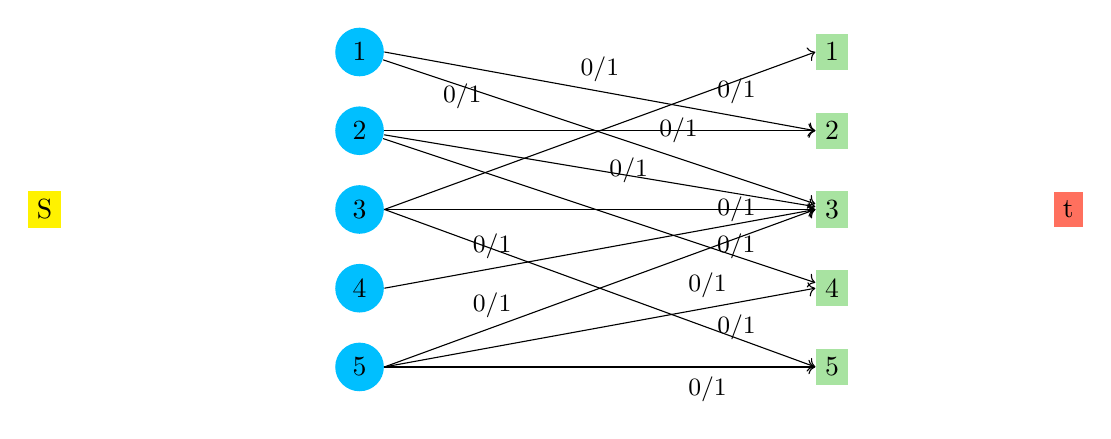
\begin{tikzpicture}
    \node[fill=yellow, rectangle](s) at (-4,-2) {S};
    \node[fill=bittersweet, rectangle](t) at (9,-2) {t};
    
    \node[fill=capri, circle] (p1) at (0,0) {1};
    \node[fill=capri, circle] (p2) at (0,-1) {2};
    \node[fill=capri, circle] (p3) at (0,-2) {3};
    \node[fill=capri, circle] (p4) at (0,-3) {4};
    \node[fill=capri, circle] (p5) at (0,-4) {5};
     
    \node[fill=grannysmithapple, rectangle] (f1) at (6,0) {1};
    \node[fill=grannysmithapple, rectangle] (f2) at (6,-1) {2};
    \node[fill=grannysmithapple, rectangle] (f3) at (6,-2) {3};
    \node[fill=grannysmithapple, rectangle] (f4) at (6,-3) {4};
    \node[fill=grannysmithapple, rectangle] (f5) at (6,-4) {5};
    
    % Potential Pairs
    \draw[->] (p1.east)--node[midway,above,font=\small]{0/1}  (f2.west);
    \draw[->] (p1) -- node[near start,left,font=\small]{0/1}  (f3);
    \draw[->] (p2) -- node[near end,left,font=\small]{0/1}  (f2);
    \draw[->] (p2) -- node[midway,right,font=\small]{0/1}  (f3);
    \draw[->] (p2) -- node[near end,right,font=\small]{0/1} (f4);
    \draw[->] (p3.east) -- node[near end,right,font=\small]{0/1}  (f1.west);
    \draw[->] (p3.east) -- node[near end,right,font=\small]{0/1}  (f3.west);
    \draw[->] (p3.east) -- node[near end,right,font=\small]{0/1}  (f5.west);
    \draw[->] (p4.east) -- node[near start,above,font=\small]{0/1}  (f3.west);
    \draw[->] (p5.east) -- node[near start,above,font=\small]{0/1} (f3.west);
    \draw[->] (p5.east) -- node[near end,below,font=\small]{0/1}  (f5.west);
    \draw[->] (p5.east) -- node[near end,above,font=\small]{0/1} (f4.west);
\end{tikzpicture}
\caption{ Two nodes (s and t) added}
\end{center}
\end{figure}

\subsection{ Add edges from source to person}

Add edges from the source to each person with flow=0 and capacity=1.Here capacity =1 means every person is allowed to take only one more item.Flow=0 means currently nobody has taken any item.

\begin{figure}[H] \begin{center}
\begin{tikzpicture}
    \node[fill=yellow, rectangle](s) at (-4,-2) {S};
    \node[fill=bittersweet, rectangle](t) at (9,-2) {t};
    
    \draw[red,->](s.east)--node[right,above,font=\small]{0/1} (p1.west);
    \draw[red,->](s.east)--node[midway,right,font=\small]{0/1} (p2.west);
    \draw[red,->](s.east)--node[midway,left,font=\small]{0/1} (p3.west);
    \draw[red,->](s.east)--node[midway,right,font=\small]{0/1} (p4.west);
    \draw[red,->](s.east)--node[midway,left,font=\small]{0/1} (p5.west);
    
    % Remaining nodes and edges
    \node[fill=capri, circle] (p1) at (0,0) {1};
    \node[fill=capri, circle] (p2) at (0,-1) {2};
    \node[fill=capri, circle] (p3) at (0,-2) {3};
    \node[fill=capri, circle] (p4) at (0,-3) {4};
    \node[fill=capri, circle] (p5) at (0,-4) {5};
     
    \node[fill=grannysmithapple, rectangle] (f1) at (6,0) {1};
    \node[fill=grannysmithapple, rectangle] (f2) at (6,-1) {2};
    \node[fill=grannysmithapple, rectangle] (f3) at (6,-2) {3};
    \node[fill=grannysmithapple, rectangle] (f4) at (6,-3) {4};
    \node[fill=grannysmithapple, rectangle] (f5) at (6,-4) {5};
    
    % Potential Pairs
    \draw[->] (p1.east)--node[midway,above,font=\small]{0/1}  (f2.west);
    \draw[->] (p1) -- node[near start,left,font=\small]{0/1}  (f3);
    \draw[->] (p2) -- node[near end,left,font=\small]{0/1}  (f2);
    \draw[->] (p2) -- node[midway,right,font=\small]{0/1}  (f3);
    \draw[->] (p2) -- node[near end,right,font=\small]{0/1} (f4);
    \draw[->] (p3.east) -- node[near end,right,font=\small]{0/1}  (f1.west);
    \draw[->] (p3.east) -- node[near end,right,font=\small]{0/1}  (f3.west);
    \draw[->] (p3.east) -- node[near end,right,font=\small]{0/1}  (f5.west);
    \draw[->] (p4.east) -- node[near start,above,font=\small]{0/1}  (f3.west);
    \draw[->] (p5.east) -- node[near start,above,font=\small]{0/1} (f3.west);
    \draw[->] (p5.east) -- node[near end,below,font=\small]{0/1}  (f5.west);
    \draw[->] (p5.east) -- node[near end,above,font=\small]{0/1} (f4.west);
\end{tikzpicture}
\caption{edges added from source to person}  \end{center} \end{figure}

\newpage

\subsection{ Add edges from food items to destination}

Add edges from food items to the destination with 0 flow and 1 capacity.Capacity is the number of copies remaining for a certain item and the flow denotes how many copies have already been taken.

\begin{figure}[H] \begin{center}
\begin{tikzpicture}
    \node[fill=yellow,rectangle](s) at (-4,-2) {S};
    \node[fill=bittersweet,rectangle](t) at (9,-2) {t};

    % Source to person
    \draw[->](s.east)--node[right,above,font=\small]{0/1} (p1.west);
    \draw[->](s.east)--node[midway,right,font=\small]{0/1} (p2.west);
    \draw[->](s.east)--node[midway,left,font=\small]{0/1} (p3.west);
    \draw[->](s.east)--node[midway,right,font=\small]{0/1} (p4.west);
    \draw[->](s.east)--node[midway,left,font=\small]{0/1} (p5.west);

    % Food items to destination
    \draw[red,->](f1.east)--node[midway,above,font=\small]{0/1} (t.west);
    \draw[red,->](f2.east)--node[midway,left,font=\small]{0/1} (t.west);
    \draw[red,->](f3.east)--node[left,right,font=\small]{0/1} (t.west);
    \draw[red,->](f4.east)--node[left,right,font=\small]{0/1} (t.west);
    \draw[red,->](f5.east)--node[left,right,font=\small]{0/1} (t.west);

    % Remaining nodes and edges
    \node[fill=capri, circle] (p1) at (0,0) {1};
    \node[fill=capri, circle] (p2) at (0,-1) {2};
    \node[fill=capri, circle] (p3) at (0,-2) {3};
    \node[fill=capri, circle] (p4) at (0,-3) {4};
    \node[fill=capri, circle] (p5) at (0,-4) {5};
     
    \node[fill=grannysmithapple, rectangle] (f1) at (6,0) {1};
    \node[fill=grannysmithapple, rectangle] (f2) at (6,-1) {2};
    \node[fill=grannysmithapple, rectangle] (f3) at (6,-2) {3};
    \node[fill=grannysmithapple, rectangle] (f4) at (6,-3) {4};
    \node[fill=grannysmithapple, rectangle] (f5) at (6,-4) {5};
    
    % Potential Pairs
    \draw[->] (p1.east)--node[midway,above,font=\small]{0/1}  (f2.west);
    \draw[->] (p1) -- node[near start,left,font=\small]{0/1}  (f3);
    \draw[->] (p2) -- node[near end,left,font=\small]{0/1}  (f2);
    \draw[->] (p2) -- node[midway,right,font=\small]{0/1}  (f3);
    \draw[->] (p2) -- node[near end,right,font=\small]{0/1} (f4);
    \draw[->] (p3.east) -- node[near end,right,font=\small]{0/1}  (f1.west);
    \draw[->] (p3.east) -- node[near end,right,font=\small]{0/1}  (f3.west);
    \draw[->] (p3.east) -- node[near end,right,font=\small]{0/1}  (f5.west);
    \draw[->] (p4.east) -- node[near start,above,font=\small]{0/1}  (f3.west);
    \draw[->] (p5.east) -- node[near start,above,font=\small]{0/1} (f3.west);
    \draw[->] (p5.east) -- node[near end,below,font=\small]{0/1}  (f5.west);
    \draw[->] (p5.east) -- node[near end,above,font=\small]{0/1} (f4.west);
\end{tikzpicture}
\caption{edges added from food items to sink}  \end{center} \end{figure}

\subsection{Reduced to Network Flow Problem}

Finally, the problem is reduced to a network flow problem where we have to apply a network flow algorithm. Here, flow \textgreater{} 0 between the pairs indicates a matching.


\begin{figure}[H] \begin{center}
    \begin{tikzpicture}
        \node[fill=yellow,rectangle](s) at (-4,-2) {S};
        \node[fill=bittersweet,rectangle](t) at (9,-2) {t};
    
        % Source to person
        \draw[->](s.east)--node[right,above,font=\small]{0/1} (p1.west);
        \draw[->](s.east)--node[midway,right,font=\small]{0/1} (p2.west);
        \draw[->](s.east)--node[midway,left,font=\small]{0/1} (p3.west);
        \draw[->](s.east)--node[midway,right,font=\small]{0/1} (p4.west);
        \draw[->](s.east)--node[midway,left,font=\small]{0/1} (p5.west);
    
        % Food items to destination
        \draw[->](f1.east)--node[midway,above,font=\small]{0/1} (t.west);
        \draw[->](f2.east)--node[midway,left,font=\small]{0/1} (t.west);
        \draw[->](f3.east)--node[left,right,font=\small]{0/1} (t.west);
        \draw[->](f4.east)--node[left,right,font=\small]{0/1} (t.west);
        \draw[->](f5.east)--node[left,right,font=\small]{0/1} (t.west);
    
        % Remaining nodes and edges
        \node[fill=capri, circle] (p1) at (0,0) {1};
        \node[fill=capri, circle] (p2) at (0,-1) {2};
        \node[fill=capri, circle] (p3) at (0,-2) {3};
        \node[fill=capri, circle] (p4) at (0,-3) {4};
        \node[fill=capri, circle] (p5) at (0,-4) {5};
         
        \node[fill=grannysmithapple, rectangle] (f1) at (6,0) {1};
        \node[fill=grannysmithapple, rectangle] (f2) at (6,-1) {2};
        \node[fill=grannysmithapple, rectangle] (f3) at (6,-2) {3};
        \node[fill=grannysmithapple, rectangle] (f4) at (6,-3) {4};
        \node[fill=grannysmithapple, rectangle] (f5) at (6,-4) {5};
        
        % Potential Pairs
        \draw[->] (p1.east)--node[midway,above,font=\small]{0/1}  (f2.west);
        \draw[->] (p1) -- node[near start,left,font=\small]{0/1}  (f3);
        \draw[->] (p2) -- node[near end,left,font=\small]{0/1}  (f2);
        \draw[->] (p2) -- node[midway,right,font=\small]{0/1}  (f3);
        \draw[->] (p2) -- node[near end,right,font=\small]{0/1} (f4);
        \draw[->] (p3.east) -- node[near end,right,font=\small]{0/1}  (f1.west);
        \draw[->] (p3.east) -- node[near end,right,font=\small]{0/1}  (f3.west);
        \draw[->] (p3.east) -- node[near end,right,font=\small]{0/1}  (f5.west);
        \draw[->] (p4.east) -- node[near start,above,font=\small]{0/1}  (f3.west);
        \draw[->] (p5.east) -- node[near start,above,font=\small]{0/1} (f3.west);
        \draw[->] (p5.east) -- node[near end,below,font=\small]{0/1}  (f5.west);
        \draw[->] (p5.east) -- node[near end,above,font=\small]{0/1} (f4.west);
    \end{tikzpicture}
    \caption{Ready to apply Max Flow Algorithm}  \end{center} \end{figure}


\pagebreak

\section{Popular Algorithms for Maximum Flow Problem}

\begin{enumerate}
    \item \textbf{Ford-Fulkerson Algorithm:}
    \begin{itemize}
        \item Uses the concept of augmenting paths to find the maximum flow.
        \item Time complexity: $O(E \cdot \text{max\_flow})$, where $E$ is the number of edges and $\text{max\_flow}$ is the maximum flow.
        \item Space complexity: $O(V)$, where $V$ is the number of vertices.
    \end{itemize}

    \item \textbf{Edmonds-Karp Algorithm (a variation of Ford-Fulkerson):}
    \begin{itemize}
        \item Utilizes BFS (Breadth-First Search) to find augmenting paths.
        \item Time complexity: $O(VE^2)$, where $V$ is the number of vertices and $E$ is the number of edges.
        \item Space complexity: $O(V^2)$, where $V$ is the number of vertices.
    \end{itemize}

    \item \textbf{Dinic's Algorithm:}
    \begin{itemize}
        \item Builds a layered network and performs multiple blocking flows.
        \item Time complexity: $O(V^2 \cdot E)$, where $V$ is the number of vertices and $E$ is the number of edges.
        \item Space complexity: $O(V^2)$, where $V$ is the number of vertices.
    \end{itemize}

    \item \textbf{Push-Relabel Algorithm:}
    \begin{itemize}
        \item Maintains a preflow that satisfies certain conditions and iteratively pushes flow along edges.
        \item Time complexity: $O(V^3)$, where $V$ is the number of vertices.
        \item Space complexity: $O(V^2)$, where $V$ is the number of vertices.
    \end{itemize}

    \item \textbf{Goldberg-Tarjan Algorithm:}
    \begin{itemize}
        \item A combination of push-relabel and relabel-to-front techniques.
        \item Time complexity: $O(V^2 \cdot E)$, where $V$ is the number of vertices and $E$ is the number of edges.
        \item Space complexity: $O(V^2)$, where $V$ is the number of vertices.
    \end{itemize}
\end{enumerate}

Among all of them,Edmonds-Karp is easier to understand and very widely used .Here,We are using Edmonds-Karp algorithm to simulate max flow problem's solution
\pagebreak
\section{Edmonds-Karp Algorithm to Solve Network Flow Problem}

The Edmonds-Karp algorithm is a popular method for finding the maximum flow in a network. It is based on the Ford-Fulkerson method and uses breadth-first search (BFS) to find augmenting paths efficiently.

\begin{algorithm}
\caption{Edmonds-Karp Algorithm}
\begin{algorithmic}[1]
\REQUIRE Network graph $G$, source node $s$, sink node $t$
\ENSURE Maximum flow $f$
\STATE Initialize flow $f(u,v) = 0$ for all edges $(u,v)$ in the graph.
\WHILE{augmenting paths exist}
    \STATE Use BFS to find the shortest augmenting path from $s$ to $t$.
    \IF{no augmenting path is found}
        \STATE Terminate the algorithm.
    \ENDIF
    \STATE Let $P$ be the augmenting path found by BFS.
    \STATE Let $cf(P)$ be the minimum residual capacity along path $P$.
    \FOR{each edge $(u,v)$ in $P$}
        \STATE Update flow $f(u,v) = f(u,v) + cf(P)$.
        \STATE Update flow $f(v,u) = f(v,u) - cf(P)$ for the reverse edge.
    \ENDFOR
\ENDWHILE
\STATE The value of the maximum flow is the sum of flow values leaving the source.
\end{algorithmic}
\end{algorithm}

This algorithm efficiently finds the maximum flow in a network by iteratively augmenting flow along the shortest augmenting paths. It terminates when no more augmenting paths can be found, guaranteeing the maximum flow is achieved.




\section{Solution}
As the algorithm uses BFS,the augmenting paths are not necessarily unique.Storing edges in different configurations may result in different valid solutions.Here we are trying to look for one of the valid solutions: 

\subsection*{Augmenting path 1}
        \begin{figure}[H] \begin{center}
		\begin{tikzpicture} 
            \node[fill=yellow,rectangle](s) at (-4,-2) {S};
            \node[fill=bittersweet,rectangle](t) at (9,-2) {t};

            \draw[brown,->](s.east)--node[right,above,font=\small]{1/1} (p1.west);
            \draw[->](s.east)--node[midway,right,font=\small]{0/1} (p2.west);
            \draw[->](s.east)--node[midway,left,font=\small]{0/1} (p3.west);
            \draw[->](s.east)--node[midway,right,font=\small]{0/1} (p4.west);
            \draw[->](s.east)--node[midway,left,font=\small]{0/1} (p5.west);


            \draw[->](f1.east)--node[midway,above,font=\small]{0/1} (t.west);
            \draw[brown,->](f2.east)--node[midway,left,font=\small]{1/1} (t.west);
            \draw[->](f3.east)--node[left,right,font=\small]{0/1} (t.west);
            \draw[->](f4.east)--node[left,right,font=\small]{0/1} (t.west);
            \draw[->](f5.east)--node[left,right,font=\small]{0/1} (t.west);


            
            \node[fill=capri, circle] (p1) at (0,0) {1};
            \node[fill=capri, circle] (p2) at (0,-1) {2};
            \node[fill=capri, circle] (p3) at (0,-2) {3};
             \node[fill=capri, circle] (p4) at (0,-3) {4};
            \node[fill=capri, circle] (p5) at (0,-4) {5};
             
            
            
            
            \node[fill=grannysmithapple, rectangle] (f1) at (6,0) {1};
            \node[fill=grannysmithapple, rectangle] (f2) at (6,-1) {2};
            \node[fill=grannysmithapple, rectangle] (f3) at (6,-2) {3};
            \node[fill=grannysmithapple, rectangle] (f4) at (6,-3) {4};
            \node[fill=grannysmithapple, rectangle] (f5) at (6,-4) {5};
            
            % Potential Pairs
            \draw[brown,->] (p1.east)--node[midway,above,font=\small]{1/1}  (f2.west);
            \draw[->] (p1) -- node[near start,left,font=\small]{0/1}  (f3);
            \draw[->] (p2) -- node[near end,left,font=\small]{0/1}  (f2);
            \draw[->] (p2) -- node[midway,right,font=\small]{0/1}  (f3);
            \draw[->] (p2) -- node[near end,right,font=\small]{0/1} (f4);
             \draw[->] (p3.east) -- node[near end,right,font=\small]{0/1}  (f1.west);
              \draw[->] (p3.east) -- node[near end,right,font=\small]{0/1}  (f3.west);
               \draw[->] (p3.east) -- node[near end,right,font=\small]{0/1}  (f5.west);
                \draw[->] (p4.east) -- node[near start,above,font=\small]{0/1}  (f3.west);
                  \draw[->] (p5.east) -- node[near start,above,font=\small]{0/1} (f3.west);
               \draw[->] (p5.east) -- node[near end,below,font=\small]{0/1}  (f5.west);
                \draw[->] (p5.east) -- node[near end,above,font=\small]{0/1} (f4.west);
            
            
            

        \end{tikzpicture}   \caption{Found augmenting path -1}  \end{center} \end{figure}
    
  Here,the flow has become 1 along the path.The bottleneck capacity=1 along the path.As a result,remaining capacity has become $1-1=0$ along the path.Therefore,the edges along the path will not be selected by BFS applied later unless any backward flow is generated.


\subsection*{Augmenting path 2}
        \begin{figure}[H] \begin{center}
		\begin{tikzpicture} 
            \node[fill=yellow,rectangle](s) at (-4,-2) {S};
            \node[fill=bittersweet,rectangle](t) at (9,-2) {t};

            \draw[brown,->](s.east)--node[right,above,font=\small]{1/1} (p1.west);
            \draw[brown,->](s.east)--node[midway,right,font=\small]{1/1} (p2.west);
            \draw[->](s.east)--node[midway,left,font=\small]{0/1} (p3.west);
            \draw[->](s.east)--node[midway,right,font=\small]{0/1} (p4.west);
            \draw[->](s.east)--node[midway,left,font=\small]{0/1} (p5.west);


            \draw[->](f1.east)--node[midway,above,font=\small]{0/1} (t.west);
            \draw[brown,->](f2.east)--node[midway,left,font=\small]{1/1} (t.west);
            \draw[->](f3.east)--node[left,right,font=\small]{0/1} (t.west);
            \draw[brown,->](f4.east)--node[left,right,font=\small]{1/1} (t.west);
            \draw[->](f5.east)--node[left,right,font=\small]{0/1} (t.west);


            
            \node[fill=capri, circle] (p1) at (0,0) {1};
            \node[fill=capri, circle] (p2) at (0,-1) {2};
            \node[fill=capri, circle] (p3) at (0,-2) {3};
             \node[fill=capri, circle] (p4) at (0,-3) {4};
            \node[fill=capri, circle] (p5) at (0,-4) {5};
             
            
            
            
            \node[fill=grannysmithapple, rectangle] (f1) at (6,0) {1};
            \node[fill=grannysmithapple, rectangle] (f2) at (6,-1) {2};
            \node[fill=grannysmithapple, rectangle] (f3) at (6,-2) {3};
            \node[fill=grannysmithapple, rectangle] (f4) at (6,-3) {4};
            \node[fill=grannysmithapple, rectangle] (f5) at (6,-4) {5};
            
            % Potential Pairs
            \draw[brown,->] (p1.east)--node[midway,above,font=\small]{1/1}  (f2.west);
            \draw[->] (p1) -- node[near start,left,font=\small]{0/1}  (f3);
            \draw[->] (p2) -- node[near end,left,font=\small]{0/1}  (f2);
            \draw[->] (p2) -- node[midway,right,font=\small]{0/1}  (f3);
            \draw[brown,->] (p2) -- node[near end,right,font=\small]{1/1} (f4);
             \draw[->] (p3.east) -- node[near end,right,font=\small]{0/1}  (f1.west);
              \draw[->] (p3.east) -- node[near end,right,font=\small]{0/1}  (f3.west);
               \draw[->] (p3.east) -- node[near end,right,font=\small]{0/1}  (f5.west);
                \draw[->] (p4.east) -- node[near start,above,font=\small]{0/1}  (f3.west);
                  \draw[->] (p5.east) -- node[near start,above,font=\small]{0/1} (f3.west);
               \draw[->] (p5.east) -- node[near end,below,font=\small]{0/1}  (f5.west);
                \draw[->] (p5.east) -- node[near end,above,font=\small]{0/1} (f4.west);
            
            
            

        \end{tikzpicture}   \caption{Found augmenting path -2}  \end{center} \end{figure}
    
    Similarly,we have found another augmenting path.Here,the bottleneck capacity is also 1.So the edges along the path are blocked for further usage.

        \subsection*{Augmenting path 3}

        \begin{figure}[H] \begin{center}
		\begin{tikzpicture} 
            \node[fill=yellow,rectangle](s) at (-4,-2) {S};
            \node[fill=bittersweet,rectangle](t) at (9,-2) {t};

            \draw[brown,->](s.east)--node[right,above,font=\small]{1/1} (p1.west);
            \draw[brown,->](s.east)--node[midway,right,font=\small]{1/1} (p2.west);
            \draw[brown,->](s.east)--node[midway,left,font=\small]{1/1} (p3.west);
            \draw[->](s.east)--node[midway,right,font=\small]{0/1} (p4.west);
            \draw[->](s.east)--node[midway,left,font=\small]{0/1} (p5.west);


            \draw[brown,->](f1.east)--node[midway,above,font=\small]{1/1} (t.west);
            \draw[brown,->](f2.east)--node[midway,left,font=\small]{1/1} (t.west);
            \draw[->](f3.east)--node[left,right,font=\small]{0/1} (t.west);
            \draw[brown,->](f4.east)--node[left,right,font=\small]{1/1} (t.west);
            \draw[->](f5.east)--node[left,right,font=\small]{0/1} (t.west);


            
            \node[fill=capri, circle] (p1) at (0,0) {1};
            \node[fill=capri, circle] (p2) at (0,-1) {2};
            \node[fill=capri, circle] (p3) at (0,-2) {3};
             \node[fill=capri, circle] (p4) at (0,-3) {4};
            \node[fill=capri, circle] (p5) at (0,-4) {5};
             
            
            
            
            \node[fill=grannysmithapple, rectangle] (f1) at (6,0) {1};
            \node[fill=grannysmithapple, rectangle] (f2) at (6,-1) {2};
            \node[fill=grannysmithapple, rectangle] (f3) at (6,-2) {3};
            \node[fill=grannysmithapple, rectangle] (f4) at (6,-3) {4};
            \node[fill=grannysmithapple, rectangle] (f5) at (6,-4) {5};
            
            % Potential Pairs
            \draw[brown,->] (p1.east)--node[midway,above,font=\small]{1/1}  (f2.west);
            \draw[->] (p1) -- node[near start,left,font=\small]{0/1}  (f3);
            \draw[->] (p2) -- node[near end,left,font=\small]{0/1}  (f2);
            \draw[->] (p2) -- node[midway,right,font=\small]{0/1}  (f3);
            \draw[brown,->] (p2) -- node[near end,right,font=\small]{1/1} (f4);
             \draw[brown,->] (p3.east) -- node[near end,right,font=\small]{1/1}  (f1.west);
              \draw[->] (p3.east) -- node[near end,right,font=\small]{0/1}  (f3.west);
               \draw[->] (p3.east) -- node[near end,right,font=\small]{0/1}  (f5.west);
                \draw[->] (p4.east) -- node[near start,above,font=\small]{0/1}  (f3.west);
                  \draw[->] (p5.east) -- node[near start,above,font=\small]{0/1} (f3.west);
               \draw[->] (p5.east) -- node[near end,below,font=\small]{0/1}  (f5.west);
                \draw[->] (p5.east) -- node[near end,above,font=\small]{0/1} (f4.west);
            
            
            

        \end{tikzpicture}   \caption{Found augmenting path -3}  \end{center} \end{figure}
    
    
This is continuation of previous steps and this step is also handled accordingly



        \subsection*{Augmenting path 4}
        \begin{figure}[H] \begin{center}
		\begin{tikzpicture} 
            \node[fill=yellow,rectangle](s) at (-4,-2) {S};
            \node[fill=bittersweet,rectangle](t) at (9,-2) {t};

            \draw[brown,->](s.east)--node[right,above,font=\small]{1/1} (p1.west);
            \draw[brown,->](s.east)--node[midway,right,font=\small]{1/1} (p2.west);
            \draw[brown,->](s.east)--node[midway,left,font=\small]{1/1} (p3.west);
            \draw[brown,->](s.east)--node[midway,right,font=\small]{1/1} (p4.west);
            \draw[->](s.east)--node[midway,left,font=\small]{0/1} (p5.west);


            \draw[brown,->](f1.east)--node[midway,above,font=\small]{1/1} (t.west);
            \draw[brown,->](f2.east)--node[midway,left,font=\small]{1/1} (t.west);
            \draw[brown,->](f3.east)--node[left,right,font=\small]{1/1} (t.west);
            \draw[brown,->](f4.east)--node[left,right,font=\small]{1/1} (t.west);
            \draw[->](f5.east)--node[left,right,font=\small]{0/1} (t.west);


            
            \node[fill=capri, circle] (p1) at (0,0) {1};
            \node[fill=capri, circle] (p2) at (0,-1) {2};
            \node[fill=capri, circle] (p3) at (0,-2) {3};
             \node[fill=capri, circle] (p4) at (0,-3) {4};
            \node[fill=capri, circle] (p5) at (0,-4) {5};
             
            
            
            
            \node[fill=grannysmithapple, rectangle] (f1) at (6,0) {1};
            \node[fill=grannysmithapple, rectangle] (f2) at (6,-1) {2};
            \node[fill=grannysmithapple, rectangle] (f3) at (6,-2) {3};
            \node[fill=grannysmithapple, rectangle] (f4) at (6,-3) {4};
            \node[fill=grannysmithapple, rectangle] (f5) at (6,-4) {5};
            
            % Potential Pairs
            \draw[brown,->] (p1.east)--node[midway,above,font=\small]{1/1}  (f2.west);
            \draw[->] (p1) -- node[near start,left,font=\small]{0/1}  (f3);
            \draw[->] (p2) -- node[near end,left,font=\small]{0/1}  (f2);
            \draw[->] (p2) -- node[midway,right,font=\small]{0/1}  (f3);
            \draw[brown,->] (p2) -- node[near end,right,font=\small]{1/1} (f4);
             \draw[brown,->] (p3.east) -- node[near end,right,font=\small]{1/1}  (f1.west);
              \draw[->] (p3.east) -- node[near end,right,font=\small]{0/1}  (f3.west);
               \draw[->] (p3.east) -- node[near end,right,font=\small]{0/1}  (f5.west);
                \draw[brown,->] (p4.east) -- node[near start,above,font=\small]{1/1}  (f3.west);
                  \draw[->] (p5.east) -- node[near start,above,font=\small]{0/1} (f3.west);
               \draw[->] (p5.east) -- node[near end,below,font=\small]{0/1}  (f5.west);
                \draw[->] (p5.east) -- node[near end,above,font=\small]{0/1} (f4.west);
            
            
            

        \end{tikzpicture}   \caption{Found augmenting path -4}  \end{center} \end{figure}
    
    This process continues to find augmenting path as long as there is a path with remaining capacity greater than 0.

        \subsection*{Augmenting path 5}

        \begin{figure}[H] \begin{center}
		\begin{tikzpicture} 
            \node[fill=yellow,rectangle](s) at (-4,-2) {S};
            \node[fill=bittersweet,rectangle](t) at (9,-2) {t};

            \draw[brown,->](s.east)--node[right,above,font=\small]{1/1} (p1.west);
            \draw[brown,->](s.east)--node[midway,right,font=\small]{1/1} (p2.west);
            \draw[brown,->](s.east)--node[midway,left,font=\small]{1/1} (p3.west);
            \draw[brown,->](s.east)--node[midway,right,font=\small]{1/1} (p4.west);
            \draw[brown,->](s.east)--node[midway,left,font=\small]{1/1} (p5.west);


            \draw[brown,->](f1.east)--node[midway,above,font=\small]{1/1} (t.west);
            \draw[brown,->](f2.east)--node[midway,left,font=\small]{1/1} (t.west);
            \draw[brown,->](f3.east)--node[left,right,font=\small]{1/1} (t.west);
            \draw[brown,->](f4.east)--node[left,right,font=\small]{1/1} (t.west);
            \draw[brown,->](f5.east)--node[left,right,font=\small]{1/1} (t.west);


            
            \node[fill=capri, circle] (p1) at (0,0) {1};
            \node[fill=capri, circle] (p2) at (0,-1) {2};
            \node[fill=capri, circle] (p3) at (0,-2) {3};
             \node[fill=capri, circle] (p4) at (0,-3) {4};
            \node[fill=capri, circle] (p5) at (0,-4) {5};
             
            
            
            
            \node[fill=grannysmithapple, rectangle] (f1) at (6,0) {1};
            \node[fill=grannysmithapple, rectangle] (f2) at (6,-1) {2};
            \node[fill=grannysmithapple, rectangle] (f3) at (6,-2) {3};
            \node[fill=grannysmithapple, rectangle] (f4) at (6,-3) {4};
            \node[fill=grannysmithapple, rectangle] (f5) at (6,-4) {5};
            
            % Potential Pairs
            \draw[brown,->] (p1.east)--node[midway,above,font=\small]{1/1}  (f2.west);
            \draw[->] (p1) -- node[near start,left,font=\small]{0/1}  (f3);
            \draw[->] (p2) -- node[near end,left,font=\small]{0/1}  (f2);
            \draw[->] (p2) -- node[midway,right,font=\small]{0/1}  (f3);
            \draw[brown,->] (p2) -- node[near end,right,font=\small]{1/1} (f4);
             \draw[brown,->] (p3.east) -- node[near end,right,font=\small]{1/1}  (f1.west);
              \draw[->] (p3.east) -- node[near end,right,font=\small]{0/1}  (f3.west);
               \draw[->] (p3.east) -- node[near end,right,font=\small]{0/1}  (f5.west);
                \draw[brown,->] (p4.east) -- node[near start,above,font=\small]{1/1}  (f3.west);
                  \draw[->] (p5.east) -- node[near start,above,font=\small]{0/1} (f3.west);
               \draw[brown,->] (p5.east) -- node[near end,below,font=\small]{1/1}  (f5.west);
                \draw[->] (p5.east) -- node[near end,above,font=\small]{0/1} (f4.west);
            
            
            

        \end{tikzpicture}   \caption{Found augmenting path -5,no more augmenting path possible}  \end{center} \end{figure}
As we can see,we have finally found all possible augmenting paths.There is no more path available with remaining capacity \textgreater{0} .\newline 
Here,the quantity of maximum flow can be obtained by two ways:
\begin{itemize}
    \item Summation of flow leaving the source node $s$:
    \[
        \sum_{v \in V} f(s, v)
    \]
    where $V$ is the set of vertices and $f(u, v)$ denotes the flow from vertex $u$ to vertex $v$.
    
    \item Summation of flow entering the sink (destination) node $t$:
    \[
        \sum_{v \in V} f(v, t)
    \]
    where $V$ is the set of vertices and $f(u, v)$ denotes the flow from vertex $u$ to vertex $v$.
\end{itemize}

Here,we find it to be equal to 5.
It implies we have become able to match 5 pairs.

\newpage


\section{Analysing the solution}

          Here,we can not augment the paths anymore.We have already found the max flow of the network.The max flow=5.Hence,Number of matching=5.
        
        \textbf{Pairs are} : 
        \begin{enumerate}
            \item Person 1,Item 2
            
            \item Person 2,Item 4
            
            \item Person 3,Item 1
            
            \item Person 4,Item 3
            
            \item Person 5,Item 5
        \end{enumerate}
        
        Using greedy approach,we found 4 pairs which is not maximum.\newline
        Thus,max flow problem helped us find an optimal solution in polynomial time.






\section{Time Complexity}
Edmond Karp's algorithm uses BFS as we need the shortest augmenting path from source to sink. Running time of BFS is $O(V + E)$ . Path search can take upto $O(V E)$ time. Some calculation and reduction leads us to a time complexity of $O((V+E)VE) = O((E)VE) = O(VE^{2})$.

\section{Extension}
Now some special cases will be discussed where the algorithm needs to be extended to solve the problem.

\newpage

\subsection{Allowing multiple items for a person}
In this case we will make the capacity of the edges  from source to person, equal to the number of items they can take. Then we can use the same algorithm to find the maximum matching. \\
For example if Person 2 is allowed to take 3 items and person 5 is allowed to take 2 items:


\begin{figure}[H] \begin{center}
    \begin{tikzpicture}
        \node[fill=yellow,rectangle](s) at (-4,-2) {S};
        \node[fill=bittersweet,rectangle](t) at (9,-2) {t};
    
        % Source to person
        \draw[->](s.east)--node[right,above,font=\small]{0/1} (p1.west);
        \draw[->](s.east)--node[midway,right,font=\small]{0/\textcolor{red}{3}} (p2.west);
        \draw[->](s.east)--node[midway,left,font=\small]{0/1} (p3.west);
        \draw[->](s.east)--node[midway,right,font=\small]{0/1} (p4.west);
        \draw[->](s.east)--node[midway,left,font=\small]{0/\textcolor{red}{2}} (p5.west);
    
        % Food items to destination
        \draw[->](f1.east)--node[midway,above,font=\small]{0/1} (t.west);
        \draw[->](f2.east)--node[midway,left,font=\small]{0/1} (t.west);
        \draw[->](f3.east)--node[left,right,font=\small]{0/1} (t.west);
        \draw[->](f4.east)--node[left,right,font=\small]{0/1} (t.west);
        \draw[->](f5.east)--node[left,right,font=\small]{0/1} (t.west);
    
        % Remaining nodes and edges
        \node[fill=capri, circle] (p1) at (0,0) {1};
        \node[fill=capri, circle] (p2) at (0,-1) {2};
        \node[fill=capri, circle] (p3) at (0,-2) {3};
        \node[fill=capri, circle] (p4) at (0,-3) {4};
        \node[fill=capri, circle] (p5) at (0,-4) {5};
         
        \node[fill=grannysmithapple, rectangle] (f1) at (6,0) {1};
        \node[fill=grannysmithapple, rectangle] (f2) at (6,-1) {2};
        \node[fill=grannysmithapple, rectangle] (f3) at (6,-2) {3};
        \node[fill=grannysmithapple, rectangle] (f4) at (6,-3) {4};
        \node[fill=grannysmithapple, rectangle] (f5) at (6,-4) {5};
        
        % Potential Pairs
        \draw[->] (p1.east)--node[midway,above,font=\small]{0/1}  (f2.west);
        \draw[->] (p1) -- node[near start,left,font=\small]{0/1}  (f3);
        \draw[->] (p2) -- node[near end,left,font=\small]{0/1}  (f2);
        \draw[->] (p2) -- node[midway,right,font=\small]{0/1}  (f3);
        \draw[->] (p2) -- node[near end,right,font=\small]{0/1} (f4);
        \draw[->] (p3.east) -- node[near end,right,font=\small]{0/1}  (f1.west);
        \draw[->] (p3.east) -- node[near end,right,font=\small]{0/1}  (f3.west);
        \draw[->] (p3.east) -- node[near end,right,font=\small]{0/1}  (f5.west);
        \draw[->] (p4.east) -- node[near start,above,font=\small]{0/1}  (f3.west);
        \draw[->] (p5.east) -- node[near start,above,font=\small]{0/1} (f3.west);
        \draw[->] (p5.east) -- node[near end,below,font=\small]{0/1}  (f5.west);
        \draw[->] (p5.east) -- node[near end,above,font=\small]{0/1} (f4.west);
    \end{tikzpicture}
    \caption{Allowing multiple item(s) for a person}  \end{center} \end{figure}


\subsection{Multiple copies of item available}
This case almost similar to the previous one. We will make the capacity of the edges from item to sink, equal to the number of copies of the item available. Then we can use the regular network flow algorithm to find the maximum matching. \\
For example if item 1 has 3 copies and item 5 has 4 copies:


\begin{figure}[H] \begin{center}
    \begin{tikzpicture}
        \node[fill=yellow,rectangle](s) at (-4,-2) {S};
        \node[fill=bittersweet,rectangle](t) at (9,-2) {t};
    
        % Source to person
        \draw[->](s.east)--node[right,above,font=\small]{0/1} (p1.west);
        \draw[->](s.east)--node[midway,right,font=\small]{0/\textcolor{red}{3}} (p2.west);
        \draw[->](s.east)--node[midway,left,font=\small]{0/1} (p3.west);
        \draw[->](s.east)--node[midway,right,font=\small]{0/1} (p4.west);
        \draw[->](s.east)--node[midway,left,font=\small]{0/\textcolor{red}{2}} (p5.west);
    
        % Food items to destination
        \draw[->](f1.east)--node[midway,above,font=\small]{0/\textcolor{red}{3}} (t.west);
        \draw[->](f2.east)--node[midway,left,font=\small]{0/1} (t.west);
        \draw[->](f3.east)--node[left,right,font=\small]{0/1} (t.west);
        \draw[->](f4.east)--node[left,right,font=\small]{0/1} (t.west);
        \draw[->](f5.east)--node[left,right,font=\small]{0/\textcolor{red}{4}} (t.west);
    
        % Remaining nodes and edges
        \node[fill=capri, circle] (p1) at (0,0) {1};
        \node[fill=capri, circle] (p2) at (0,-1) {2};
        \node[fill=capri, circle] (p3) at (0,-2) {3};
        \node[fill=capri, circle] (p4) at (0,-3) {4};
        \node[fill=capri, circle] (p5) at (0,-4) {5};
         
        \node[fill=grannysmithapple, rectangle] (f1) at (6,0) {1};
        \node[fill=grannysmithapple, rectangle] (f2) at (6,-1) {2};
        \node[fill=grannysmithapple, rectangle] (f3) at (6,-2) {3};
        \node[fill=grannysmithapple, rectangle] (f4) at (6,-3) {4};
        \node[fill=grannysmithapple, rectangle] (f5) at (6,-4) {5};
        
        % Potential Pairs
        \draw[->] (p1.east)--node[midway,above,font=\small]{0/1}  (f2.west);
        \draw[->] (p1) -- node[near start,left,font=\small]{0/1}  (f3);
        \draw[->] (p2) -- node[near end,left,font=\small]{0/1}  (f2);
        \draw[->] (p2) -- node[midway,right,font=\small]{0/1}  (f3);
        \draw[->] (p2) -- node[near end,right,font=\small]{0/1} (f4);
        \draw[->] (p3.east) -- node[near end,right,font=\small]{0/1}  (f1.west);
        \draw[->] (p3.east) -- node[near end,right,font=\small]{0/1}  (f3.west);
        \draw[->] (p3.east) -- node[near end,right,font=\small]{0/1}  (f5.west);
        \draw[->] (p4.east) -- node[near start,above,font=\small]{0/1}  (f3.west);
        \draw[->] (p5.east) -- node[near start,above,font=\small]{0/1} (f3.west);
        \draw[->] (p5.east) -- node[near end,below,font=\small]{0/1}  (f5.west);
        \draw[->] (p5.east) -- node[near end,above,font=\small]{0/1} (f4.west);
    \end{tikzpicture}
    \caption{Multiple copies of items available}  \end{center} \end{figure}


\subsection{Taking same item multiple times}
We have to make the edges from person to item have capacity, the number of times that particular person can take that particular item. Then we can use our network flow algorithm to solve the problem. \\
For example if Person1 can take Item 2 upto 5 times:


\begin{figure}[H] \begin{center}
    \begin{tikzpicture}
        \node[fill=yellow,rectangle](s) at (-4,-2) {S};
        \node[fill=bittersweet,rectangle](t) at (9,-2) {t};
    
        % Source to person
        \draw[->](s.east)--node[right,above,font=\small]{0/1} (p1.west);
        \draw[->](s.east)--node[midway,right,font=\small]{0/\textcolor{red}{3}} (p2.west);
        \draw[->](s.east)--node[midway,left,font=\small]{0/1} (p3.west);
        \draw[->](s.east)--node[midway,right,font=\small]{0/1} (p4.west);
        \draw[->](s.east)--node[midway,left,font=\small]{0/\textcolor{red}{2}} (p5.west);
    
        % Food items to destination
        \draw[->](f1.east)--node[midway,above,font=\small]{0/\textcolor{red}{3}} (t.west);
        \draw[->](f2.east)--node[midway,left,font=\small]{0/1} (t.west);
        \draw[->](f3.east)--node[left,right,font=\small]{0/1} (t.west);
        \draw[->](f4.east)--node[left,right,font=\small]{0/1} (t.west);
        \draw[->](f5.east)--node[left,right,font=\small]{0/\textcolor{red}{4}} (t.west);
    
        % Remaining nodes and edges
        \node[fill=capri, circle] (p1) at (0,0) {1};
        \node[fill=capri, circle] (p2) at (0,-1) {2};
        \node[fill=capri, circle] (p3) at (0,-2) {3};
        \node[fill=capri, circle] (p4) at (0,-3) {4};
        \node[fill=capri, circle] (p5) at (0,-4) {5};
         
        \node[fill=grannysmithapple, rectangle] (f1) at (6,0) {1};
        \node[fill=grannysmithapple, rectangle] (f2) at (6,-1) {2};
        \node[fill=grannysmithapple, rectangle] (f3) at (6,-2) {3};
        \node[fill=grannysmithapple, rectangle] (f4) at (6,-3) {4};
        \node[fill=grannysmithapple, rectangle] (f5) at (6,-4) {5};
        
        % Potential Pairs
        \draw[->] (p1.east)--node[midway,above,font=\small]{0/\textcolor{red}{5}}  (f2.west);
        \draw[->] (p1) -- node[near start,left,font=\small]{0/1}  (f3);
        \draw[->] (p2) -- node[near end,left,font=\small]{0/1}  (f2);
        \draw[->] (p2) -- node[midway,right,font=\small]{0/1}  (f3);
        \draw[->] (p2) -- node[near end,right,font=\small]{0/1} (f4);
        \draw[->] (p3.east) -- node[near end,right,font=\small]{0/1}  (f1.west);
        \draw[->] (p3.east) -- node[near end,right,font=\small]{0/1}  (f3.west);
        \draw[->] (p3.east) -- node[near end,right,font=\small]{0/1}  (f5.west);
        \draw[->] (p4.east) -- node[near start,above,font=\small]{0/1}  (f3.west);
        \draw[->] (p5.east) -- node[near start,above,font=\small]{0/1} (f3.west);
        \draw[->] (p5.east) -- node[near end,below,font=\small]{0/1}  (f5.west);
        \draw[->] (p5.east) -- node[near end,above,font=\small]{0/1} (f4.west);
    \end{tikzpicture}
    \caption{Allowed to take same item multiple times}  \end{center} \end{figure}
        

\section{References}
\bibliographystyle{plain}
\bibliography{ref}

\end{document}